\documentclass{standalone}
\usepackage{pgfplots}
\pgfplotsset{compat=1.18}
\usepgfplotslibrary{colorbrewer}
\pgfplotsset{cycle list/Set1-6}

\begin{document}

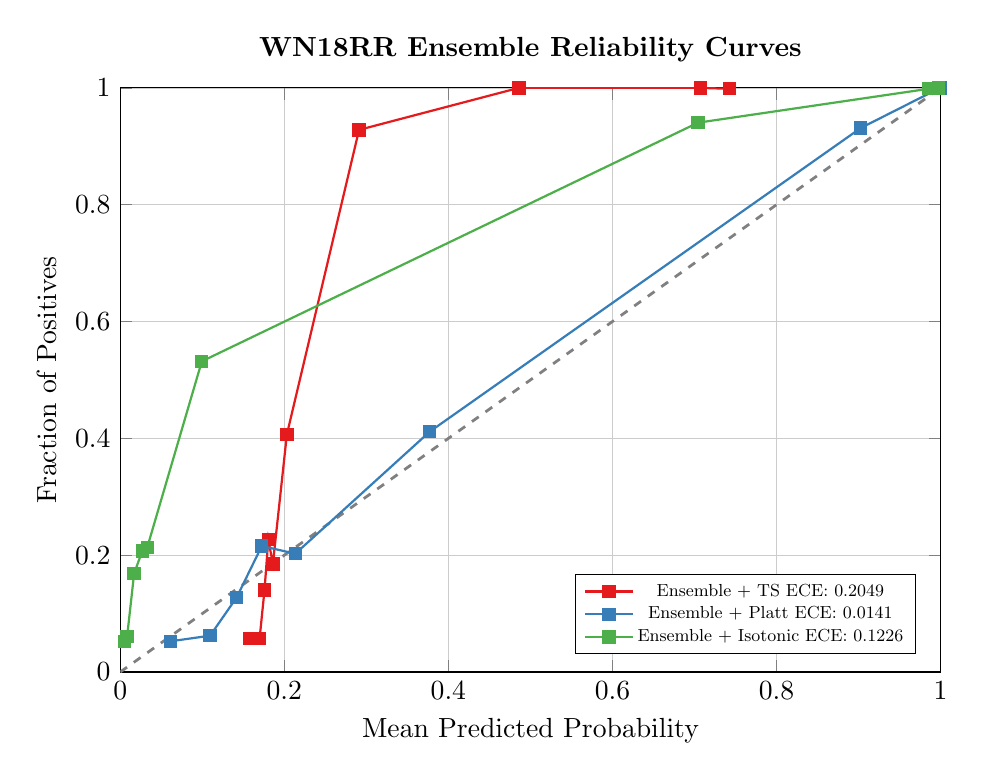
\begin{tikzpicture}
\begin{axis}[
    title={\textbf{WN18RR Ensemble Reliability Curves}},
    xlabel={Mean Predicted Probability},
    ylabel={Fraction of Positives},
    xmin=0, xmax=1,
    ymin=0, ymax=1,
    xtick={0, 0.2, 0.4, 0.6, 0.8, 1.0},
    ytick={0, 0.2, 0.4, 0.6, 0.8, 1.0},
    legend pos= south east,
    legend style={nodes={scale=0.7, transform shape}, font=\small},
    grid=both,
    grid style={line width=.1pt, draw=gray!20},
    major grid style={line width=.2pt, draw=gray!40},
    width=12cm,
    height=9cm,
    cycle list name=Set1-6
]

% Perfectly Calibrated Line
\addplot [color=gray, dashed, line width=1pt, forget plot]
    coordinates {(0,0)(1,1)};


\addplot+[mark=square*, thick] coordinates { (0.15775501, 0.05741627) (0.16986108, 0.05741627) (0.17584712, 0.14035088) (0.18047062, 0.22683706) (0.18604459, 0.18500797) (0.20310769, 0.40669856) (0.29109635, 0.92811502) (0.48590021, 1.00000000) (0.70691116, 1.00000000) (0.74293832, 0.99840510) }; \addlegendentry{Ensemble + TS ECE: 0.2049}

\addplot+[mark=square*, thick] coordinates { (0.06146737, 0.05263158) (0.10953045, 0.06220096) (0.14186112, 0.12759171) (0.17252283, 0.21565495) (0.21340922, 0.20255183) (0.37726620, 0.41148325) (0.90265927, 0.93130990) (0.99942355, 1.00000000) (0.99999988, 0.99840383) }; \addlegendentry{Ensemble + Platt ECE: 0.0141}

\addplot+[mark=square*, thick] coordinates { (0.00513100, 0.05263158) (0.00835144, 0.06074766) (0.01691122, 0.16855204) (0.02686185, 0.20736698) (0.03290856, 0.21333333) (0.09942230, 0.53186275) (0.70429318, 0.94040698) (0.98599061, 0.99853694) (0.99758111, 1.00000000) }; \addlegendentry{Ensemble + Isotonic ECE: 0.1226}


\end{axis}
\end{tikzpicture}

\end{document}